%%%%%%%%%%%%%%%%%%%%%%%%%%%%%%%%%%%%%%%%%%%%%
\section{Initial data far from equilibrium}
\label{Sec:FarFromEq}
%%%%%%%%%%%%%%%%%%%%%%%%%%%%%%%%%%%%%%%%%%%%%

In this section we consider the gas cloud~(\ref{Eq:Pulse}), which is concentrated about one orbital phase and is far from any steady state, and we analyze how its evolution changes when its mass is increased. We start with the simulations and with a parameter $\mu$ which compares the amplitude of the potential generated by the cloud with the spread of its orbital frequencies. Next, we describe the evolution of the cloud for increasing values of $\mu$: for small $\mu$ the cloud mixes; for larger $\mu$ a compact part of it survives as a dense core at the circular orbit, whose radial oscillation is damped; and above a critical value of $\mu$ this oscillation persists, such that the potential does not relax. Then, we characterize the state of the gas at late times, and finally we analyze the dependence of these results on the widths of the cloud and on the external potential.


\subsection{Simulations and the parameter $\mu$}
\label{SubSec:FarRuns}

The reference family of simulations consists of the cloud~(\ref{Eq:Pulse}) with $\sigma_Q = \sigma_J = 0.1$ and $L_0 = 2$ in the isochrone potential, with the masses $M_{gas}/M = 10^{-3}$, $0.01$, $0.015$, $0.02$, $0.025$, $0.03$, $0.04$, $0.05$, $0.07$, $0.1$ and $0.3$, together with a simulation without self-gravity. In order to analyze the dependence on the shape of the cloud, we vary its width in angle, $\sigma_Q = 0.2$ and $0.4$ with $M_{gas}/M = 0.01$, $0.02$, $0.04$ and $0.08$, and its width in action, $\sigma_J = 0.05$ with $M_{gas}/M = 0.005$, $0.01$ and $0.02$ and $\sigma_J = 0.2$ with $M_{gas}/M = 0.02$, $0.04$ and $0.08$. Finally, we consider the cloud with $\sigma_Q = \sigma_J = 0.1$ in the Kepler potential, with $M_{gas}/M = 0.01$, $0.02$, $0.04$ and $0.08$. This is the external potential of the nonlinear phase mixing result of Ref.~\cite{sCjL26}, although the reduced model and the support of the DF, which extends to the circular orbit, differ from the assumptions made there. The simulations use the lattice~(\ref{Eq:Lattice}) with $N_J\times N_Q = 400\times 25$, except for $\sigma_Q = 0.2$ ($N_Q = 50$) and $\sigma_J = 0.2$ ($N_J = 800$), and the time step $\Delta t = 0.05$, and they extend to $t = 10^4$ ($2\times 10^4$ for $\sigma_J = 0.05$). In order to test the convergence, we have repeated the simulations of the reference family with $M_{gas}/M = 0.01$, $0.02$ and $0.1$ with $N_Q = 100$, and the one with $M_{gas}/M = 0.01$ with $N_J = 800$. In all the simulations the gas particles remain bound, and the observables are computed with the action-angle variables of the instantaneous potential and the weight function $B = 1$, see sections~\ref{SubSec:Observables} and~\ref{SubSec:PIC}.

In the absence of self-gravity the cloud mixes on a time scale which is set by the spread of its orbital frequencies. We characterize this spread by the interval $[\underline{J},\overline{J}]$ in which the factor $J^2\exp(-J^2/\sigma_J^2)$ of the DF~(\ref{Eq:Pulse}) exceeds one percent of its maximum, by its width $\Delta J := \overline{J} - \underline{J}$, and by the width $\Delta\Omega := \Omega(\underline{J}) - \Omega(\overline{J})$ of the corresponding frequency band of the external potential. After the time
\begin{equation}
\tau_1 := \frac{2\pi}{\Delta\Omega}
\label{Eq:tau1}
\end{equation}
the orbits at the two ends of this interval have drifted apart by one revolution, such that the first harmonic of the cloud has been spread over the orbit. For $\sigma_Q = \sigma_J = 0.1$ in the isochrone potential one has $\Delta J = 0.270$, $[\Omega(\overline{J}),\Omega(\underline{J})] = [0.0513,0.0705]$ and $\tau_1 = 327$, for $\sigma_J = 0.05$ and $0.2$ one has $\tau_1 = 589$ and $198$, respectively, and in the Kepler potential $\tau_1 = 161$. Hence, the simulations extend over at least $30$ units of $\tau_1$.

The self-gravity of the cloud couples the motions of its particles and acts against the mixing. In order to compare both effects, consider the motion of the gas particles relative to the center of the cloud. In the absence of self-gravity, the angle variable of a particle relative to the one of the center drifts with a velocity which varies by $\Delta\Omega$ across the support of the cloud. Approximating the derivative of the frequency by the constant $|\Omega'| = \Delta\Omega/\Delta J$, the energy which is associated with this differential drift, $|\Omega'|(J - J_c)^2/2$ with $J_c$ the action variable of the center, is of the order of $\Delta\Omega\,\Delta J$. On the other hand, the strength of the self-gravity is measured by the amplitude $A$ of the variation of the potential which is generated by the cloud. This suggests the parameter
\begin{equation}
\mu := \left( \frac{A}{\Delta\Omega\,\Delta J} \right)^{1/2} = \frac{\omega_b}{\Delta\Omega},\qquad
\omega_b := \left( |\Omega'| A \right)^{1/2},
\label{Eq:muDef}
\end{equation}
whose square compares these two energies, and one expects the self-gravity of the cloud to modify the mixing when $\mu$ is of order one. The frequency $\omega_b$ is the frequency of the small oscillations of a pendulum with the Hamiltonian $|\Omega'|(J - J_c)^2/2 - A\cos\vartheta$, which describes the trapping of particles by a wave in a plasma~\cite{tO65}; in terms of $\mu$, $2\pi/\omega_b = \tau_1/\mu$. This argument is a heuristic one: it does not describe how the potential of the cloud depends on the positions of its particles, and it does not predict the critical value of $\mu$. We measure $A$ as half of the largest variation of $\Phi_{gas}(t,r)$ at fixed $r$ during the first radial period $0\leq t\leq 2\pi/\Omega(\overline{J})$, maximized over $3\leq r\leq 15$. For small masses $A$ is determined by the initial datum: in the reference family with $M_{gas}/M\leq 0.025$ it differs by less than $5$ percent from $0.0496\, M_{gas}/M$, where $0.0496$ is the amplitude, per unit mass, of the potential which the cloud generates when it moves in the external potential alone. Hence, $\mu$ grows like $(M_{gas}/M)^{1/2}$. For $M_{gas}/M = 10^{-3}$, $0.01$, $0.1$ and $0.3$ one has $\mu = 0.10$, $0.31$, $0.89$ and $1.16$, respectively.


\subsection{Evolution of the cloud}
\label{SubSec:FarRegimes}

\begin{figure}[htp]
\centerline{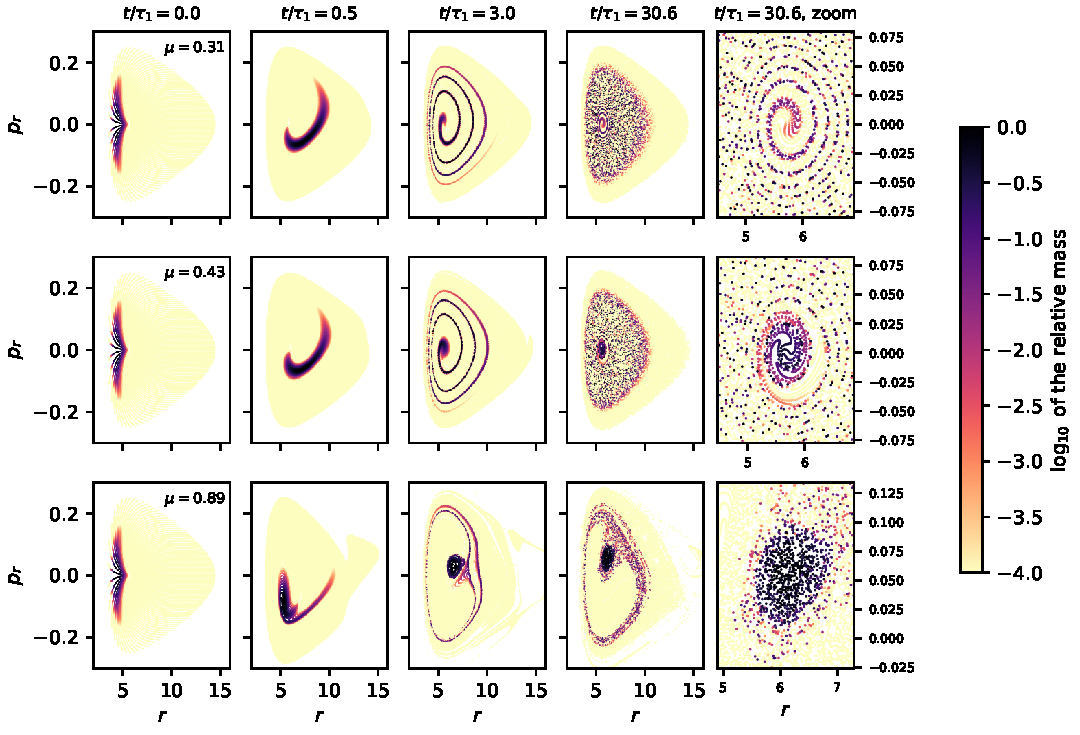
\includegraphics[width=\textwidth]{figuras/bulto_fase.pdf}}
\caption{The computational particles in the $(r,p_r)$-plane at four different times for the cloud~(\ref{Eq:Pulse}) with $\sigma_Q = \sigma_J = 0.1$ in the isochrone potential, for $M_{gas}/M = 0.01$, $0.02$ and $0.1$ (from top to bottom; $N_J\times N_Q = 400\times 100$). The color indicates the mass of each particle relative to the largest one. The last column shows, at the final time, the neighborhood of the circular orbit (upper two rows) and of the core (lower row). For $\mu = 0.31$ the cloud mixes, for $\mu = 0.43$ a dense core is left at the circular orbit, and for $\mu = 0.89$ the core oscillates radially until the end of the simulation.}
\label{Fig:CloudPhase}
\end{figure}

Figure~\ref{Fig:CloudPhase} shows the computational particles in the $(r,p_r)$-plane for three clouds of the reference family. For $M_{gas}/M = 0.01$ ($\mu = 0.31$) the evolution resembles the mixing without self-gravity of Fig.~\ref{Fig:Pulse}: the cloud is sheared into a spiral which winds up around the circular orbit, and at $t = 30\tau_1$ the gas fills the region of phase space which is covered by its orbits. For $M_{gas}/M = 0.02$ ($\mu = 0.43$) most of the gas evolves in the same way, but a compact part of the cloud ends up at the circular orbit, where it forms a dense core which is visible from $t = 3\tau_1$ on. For $M_{gas}/M = 0.1$ ($\mu = 0.89$) about half of the cloud contracts within the first radial periods into a core which is not at rest: for $t\geq 15\tau_1$ its center moves between $r = 4.7$ and $r = 6.7$ with the frequency $0.074$, which is close to the frequency $\Omega(0) = 0.0711$ of the circular orbit in the external potential, while the root mean square distance of its particles from the center is $0.17$. The rest of the gas is mixed around it.

\begin{figure}[htp]
\centerline{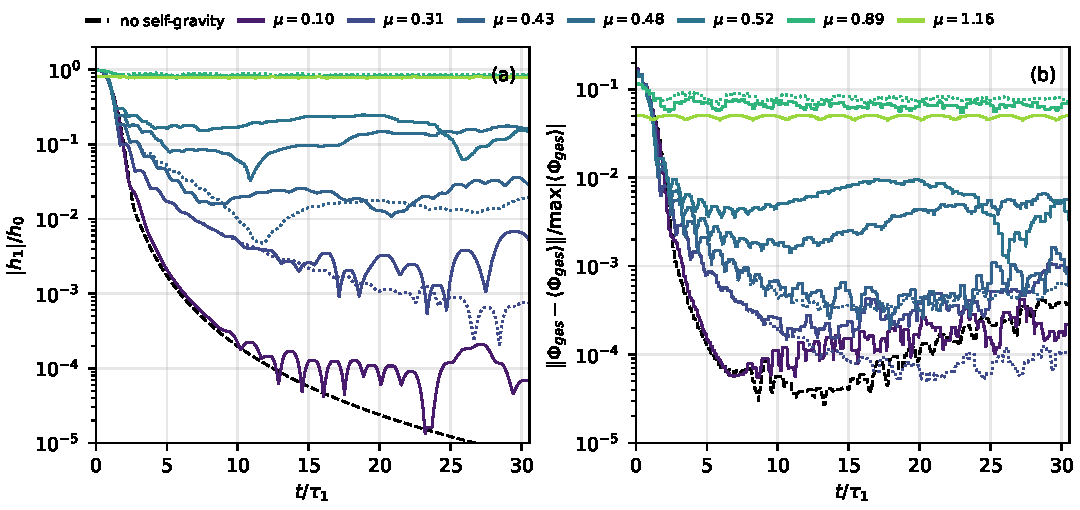
\includegraphics[width=\textwidth]{figuras/bulto_series.pdf}}
\caption{Evolution of the cloud~(\ref{Eq:Pulse}) with $\sigma_Q = \sigma_J = 0.1$ in the isochrone potential for different masses, labeled by the value of $\mu$. (a) Envelope of $|h_1|/h_0$ (largest value in a moving window of width $100$), computed with the action-angle variables of the instantaneous potential, for $N_J\times N_Q = 400\times 25$ (solid lines) and $400\times 100$ (dotted lines). (b) Deviation of the potential generated by the gas from its average over the second half of the simulation, measured with the norm~(\ref{Eq:deltaPhiNorm}) over $3\leq r\leq 15$ in units of the largest value of $|\langle\Phi_{gas}\rangle|$ (envelope as in (a)). The potential is computed from the radii of the particles; without self-gravity (dashed line) it is the potential which the gas would generate if it acted on itself.}
\label{Fig:CloudSeries}
\end{figure}

The function $|h_1(t)|/h_0$ and the oscillation of the potential are shown in Fig.~\ref{Fig:CloudSeries} for the reference family. Without self-gravity, $|h_1|$ decays like $t^{-3}$ (a fit of the envelope over $10\leq t/\tau_1\leq 30$ gives the exponent $-3.03$), which is the analogue of the tail~(\ref{Eq:Tail}) for the endpoint $J = 0$ of the support, at which $\hat{F}_1$ vanishes like $J^2$. With self-gravity the decay slows down, and the level which is reached at late times increases with $\mu$. Averaged over $10\leq t/\tau_1\leq 20$, $|h_1|/h_0$ is $1.1\times 10^{-4}$, $2.4\times 10^{-3}$ and $1.2\times 10^{-2}$ for $\mu = 0.10$, $0.31$ and $0.43$ (the last two values for $N_Q = 100$), compared to $7.0\times 10^{-5}$ without self-gravity, and it lies between $0.09$ and $0.85$ for $\mu\geq 0.48$.

The potential which is generated by the gas behaves in the same way, see Fig.~\ref{Fig:CloudSeries}(b). Without self-gravity, the potential which the gas would generate relaxes to its final profile through the mixing alone: its deviation~(\ref{Eq:deltaPhi}) from the average over the second half of the simulation falls below $10^{-3}$ of the largest value of $|\langle\Phi_{gas}\rangle|$ at $t = 2.9\tau_1$. With self-gravity and $\mu\leq 0.43$ the potential still relaxes, but more slowly: the same level is reached at $t = 3.3\tau_1$, $4.8\tau_1$, $5.5\tau_1$ and $6.2\tau_1$ for $\mu = 0.10$, $0.31$, $0.37$ and $0.43$, respectively. Over $10\leq t/\tau_1\leq 20$ the deviation lies between $7\times 10^{-5}$ and $3\times 10^{-4}$, compared to $4\times 10^{-5}$ without self-gravity, and it is reduced when the number of particles is increased (dotted lines). For $\mu\geq 0.48$, in contrast, the deviation never falls below $10^{-3}$: over $10\leq t/\tau_1\leq 20$ it lies between $1.6\times 10^{-3}$ and $4.6\times 10^{-2}$, since the potential oscillates with the core. Therefore, for $\mu\leq 0.43$ the gravitational field generated by the gas relaxes to a stationary field while the DF continues to mix, which is the analogue of Landau damping, whereas for $\mu\geq 0.48$ the field does not relax. (Without self-gravity the deviation increases again for $t\gtrsim 15\tau_1$, which we attribute to the spurious recurrence~(\ref{Eq:Recurrence}) of the higher harmonics of the potential on the lattice; for $n = 10$ the recurrence time is about $4800\approx 15\tau_1$.)


\subsection{The state at late times: dense core and its oscillation}
\label{SubSec:FarLate}

In the absence of self-gravity the gas relaxes to the angle average $\hat{F}_0(J)$ of the initial DF, see section~\ref{Sec:Linear}. For the cloud~(\ref{Eq:Pulse}), Eq.~(\ref{Eq:PulseFourier}) gives $\hat{F}_0(J) = \alpha\, e^{-z} I_0(z) J^2\exp(-J^2/\sigma_J^2)$, whose maximum $\hat{F}_{max} = \alpha\, e^{-z} I_0(z)\sigma_J^2/e$ is attained at $J = \sigma_J$. This is the largest value of the DF which can be reached anywhere by mixing the cloud at fixed action. It is much smaller than the maximum $F_{max} = \alpha\sigma_J^2/e$ of the initial DF itself: $F_{max}/\hat{F}_{max} = 17.7$, $8.8$ and $4.2$ for $\sigma_Q = 0.1$, $0.2$ and $0.4$, respectively. In order to characterize the state which is reached with self-gravity, we compute the average of the DF over the angle variable of the instantaneous potential, as a function of the action variable of the same potential, from the mass of the computational particles in a set of intervals of $J$, and we average the result over $t\geq 20\tau_1$.

\begin{figure}[htp]
\centerline{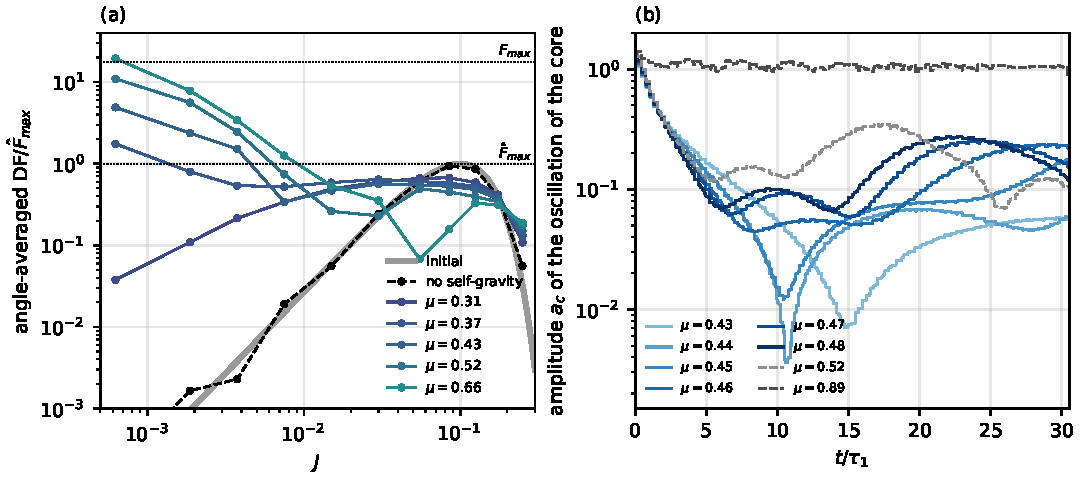
\includegraphics[width=\textwidth]{figuras/bulto_estado.pdf}}
\caption{State of the cloud~(\ref{Eq:Pulse}) with $\sigma_Q = \sigma_J = 0.1$ in the isochrone potential at late times. (a) Angle average of the DF as a function of the action variable of the instantaneous potential, averaged over $t\geq 20\tau_1$, in units of the maximum $\hat{F}_{max}$ of the angle average of the initial DF (thick gray line). The dotted lines indicate $\hat{F}_{max}$ and the maximum $F_{max}$ of the initial DF. The results refer to $N_Q = 100$ for $\mu = 0.31$ and $0.43$ and to $N_Q = 25$ otherwise. (b) Amplitude $a_c$ of the radial oscillation of the core (see the text), for $N_Q = 25$ (solid lines) and $N_Q = 100$ (dotted lines).}
\label{Fig:CloudState}
\end{figure}

The result is shown in Fig.~\ref{Fig:CloudState}(a). Without self-gravity the angle average of the DF does not change, as it should. For $\mu = 0.31$ it remains a smooth function which lies below $\hat{F}_{max}$ everywhere (its largest value is $0.67\,\hat{F}_{max}$), but it differs from $\hat{F}_0$: the region near the circular orbit, where the initial DF vanishes like $J^2$, has been partially filled. The fraction of the mass of the gas with $J < 0.2\sigma_J$ is $6.1$ percent, compared to $0.5$ percent without self-gravity. Hence, although the gas mixes, the state which it reaches is not the angle average of the initial DF. The reason is that during the first few units of $\tau_1$ the potential of the cloud oscillates with the orbital period of its particles, such that their action variables are not conserved; the fraction quoted above grows from $1.0$ to $5.8$ percent between $t = 0$ and $t = 3\tau_1$ and changes by less than $0.3$ percent afterwards. This fraction increases continuously with $\mu$, see Table~\ref{Tab:CloudState}, and it is the same for the three lattices which we have used for $\mu = 0.31$ ($6.0$, $6.1$ and $6.1$ percent).

For $\mu\geq 0.37$ a peak develops at the circular orbit which exceeds $\hat{F}_{max}$. In the interval $J < 0.025\sigma_J$ the angle average of the DF is $1.3\,\hat{F}_{max}$ for $\mu = 0.37$, about $4\,\hat{F}_{max}$ for $\mu = 0.43$ ($4.3$ and $3.6$ with $N_Q = 25$ and $100$), and $8.3$ and $13.6\,\hat{F}_{max}$ for $\mu = 0.52$ and $0.66$; in the innermost interval of Fig.~\ref{Fig:CloudState}(a) it reaches $F_{max}$ for $\mu = 0.66$, within the sampling error. Values above $\hat{F}_{max}$ cannot be obtained by mixing the cloud at fixed action. They show that part of the dense cloud has been transported to the circular orbit before it was mixed. A distribution which is centered at the circular orbit is not dispersed by the differential rotation of the orbits about it, which only winds up its internal structure (see the last column of Fig.~\ref{Fig:CloudPhase}). We refer to this part of the gas as the core.

\begin{table}[htp]
\begin{center}
\begin{tabular}{ll|c|c|cc|cc}
\hline\hline
 & & & mass with & & & \multicolumn{2}{c}{$a_c$ for $t/\tau_1$ in} \\
$M_{gas}/M$ & $\mu$ & $|h_1|/h_0$ & $J < 0.2\sigma_J$ & $m_c$ & $m_c/m_{mix}$ & $[1,2]$ & $[20,30]$ \\
\hline
$0$ & $0$ & $7.0\times 10^{-5}$ & $0.005$ & $0.051$ & $1.2$ & -- & -- \\
$0.001$ & $0.10$ & $1.1\times 10^{-4}$ & $0.007$ & $0.048$ & $1.2$ & -- & -- \\
$0.01$ & $0.31$ & $2.4\times 10^{-3}$ & $0.061$ & $0.031$ & $0.7$ & -- & -- \\
$0.015$ & $0.37$ & $8.5\times 10^{-3}$ & $0.108$ & $0.040$ & $1.0$ & -- & -- \\
$0.02$ & $0.43$ & $1.2\times 10^{-2}$ & $0.160$ & $0.103$ & $2.5$ & $0.51$ & $0.06$ \\
$0.025$ & $0.48$ & $0.091$ & $0.225$ & $0.173$ & $4.2$ & $0.55$ & $0.27$ \\
$0.03$ & $0.52$ & $0.22$ & $0.276$ & $0.232$ & $5.6$ & $0.55$ & $0.24$ \\
$0.04$ & $0.60$ & $0.32$ & $0.377$ & $0.337$ & $8.1$ & $0.57$ & $0.29$ \\
$0.05$ & $0.66$ & $0.19$ & $0.450$ & $0.376$ & $9.1$ & $0.49$ & $0.24$ \\
$0.07$ & $0.76$ & $0.58$ & $0.557$ & $0.479$ & $11.5$ & $0.93$ & $0.58$ \\
$0.1$ & $0.89$ & $0.85$ & $0.290$ & $0.516$ & $12.4$ & $1.00$ & $0.99$ \\
$0.3$ & $1.16$ & $0.69$ & $0.749$ & $0.471$ & $11.3$ & $0.59$ & $0.63$ \\
\hline\hline
\end{tabular}
\end{center}
\caption{State at late times of the cloud~(\ref{Eq:Pulse}) with $\sigma_Q = \sigma_J = 0.1$ in the isochrone potential: mean value of $|h_1|/h_0$ over $10\leq t/\tau_1\leq 20$; fraction of the mass of the gas whose action variable with respect to the instantaneous potential is smaller than $0.2\sigma_J$, and fraction $m_c$ inside the ellipse~(\ref{Eq:CoreEllipse}) about the maximum of the density, both averaged over $t\geq 20\tau_1$; and half of the difference between the largest and the smallest radius of the center of the core in the first and in the last time interval. For a gas which is mixed at fixed action $m_c\leq m_{mix} = 0.042$, and no amplitude is given when $m_c$ is compatible with this bound. For $\mu = 0.89$ the core does not lie at the circular orbit, which explains the smaller value in the fourth column. The rows with $\mu = 0.31$, $0.43$ and $0.89$ refer to $N_Q = 100$.}
\label{Tab:CloudState}
\end{table}

In order to follow the core also when it is not at rest, we determine at each time the maximum $(r_*,p_*)$ of the density of the gas in the $(r,p_r)$-plane and consider the ellipse
\begin{equation}
\frac{(r - r_*)^2}{a^2} + \frac{(p_r - p_*)^2}{\kappa^2 a^2} < 1,\qquad
a := \left( \frac{2J_*}{\kappa} \right)^{1/2},\qquad J_* := 0.05\,\sigma_J,
\label{Eq:CoreEllipse}
\end{equation}
where $\kappa := \Omega(0)$ is the frequency of the circular orbit of the external potential. In the harmonic approximation this is the set of orbits about $(r_*,p_*)$ whose action variable is smaller than $J_*$; for $\sigma_J = 0.1$ in the isochrone potential $a = 0.38$. We denote by $m_c$ the fraction of the mass of the gas inside this ellipse, averaged over $t\geq 20\tau_1$. Since the area of the ellipse is $2\pi J_*$, a gas which is mixed at fixed action satisfies $m_c\leq m_{mix}$, where $m_{mix} = 0.05\cdot 4/(e\sqrt{\pi}) = 0.042$ is the mass fraction which corresponds to the density $\hat{F}_{max}$, independently of $\sigma_Q$ and $\sigma_J$; hence, $m_c/m_{mix}$ is the mean value of the DF in the ellipse in units of $\hat{F}_{max}$. As shown in Table~\ref{Tab:CloudState}, $m_c/m_{mix}$ lies between $0.7$ and $1.2$ for $\mu\leq 0.37$, which is compatible with one within the fluctuations due to the finite number of particles, and it grows from $2.5$ for $\mu = 0.43$ to about $12$ for $\mu\geq 0.76$. For $\mu = 0.43$ the core contains $10$ percent of the mass of the gas, and for $\mu = 0.89$ at least $52$ percent; for the largest masses the core is larger than the ellipse, such that $m_c$ is a lower bound.

The oscillation of the core is described by the mean radius $r_c(t)$ of the computational particles which lie inside the ellipse at the end of the simulation. We denote by $a_c(t)$ the envelope of the deviation of $r_c$ from its average over one radial period; it is shown in Fig.~\ref{Fig:CloudState}(b). In all the simulations with a core, $a_c$ lies between $0.2$ and $1.1$ at $t = 2\tau_1$. Its subsequent behavior depends on $\mu$. For $\mu = 0.43$ the oscillation is damped: $a_c$ decays from $0.41$ at $t = 2\tau_1$ to less than $7\times 10^{-3}$ at $t\approx 15\tau_1$ to $18\tau_1$, and a fit of an exponential function in the interval $2\leq t/\tau_1\leq 14$ gives the decay times $3.8\tau_1$ and $4.7\tau_1$ for $N_Q = 100$ and $N_Q = 25$, respectively. Afterwards $a_c$ increases again, to $0.06$ at the end of both simulations, which is $15$ percent of its value at $t = 2\tau_1$ and less than half of the size of the core, whose root mean square radial extension is $0.15$. For $0.48\leq\mu\leq 0.66$ the first decay stops at $t\approx 4\tau_1$ to $9\tau_1$, when $a_c$ has decreased by a factor between $3$ and $12$, and afterwards $a_c$ is modulated, with maxima between $0.2$ and $0.35$ and minima between $0.02$ and $0.2$, without an overall decay until the end of the simulations. For $\mu = 0.76$ it remains above $0.39$, and for $\mu\geq 0.89$ it does not decay. Therefore, the change between $\mu = 0.43$ and $\mu = 0.48$ which was found in the previous subsection separates the clouds whose core settles down at the circular orbit from those whose core keeps oscillating. The former reach a state which is stationary up to the small residual oscillation mentioned above, and which consists of a core and of mixed gas around it; the damping of the oscillation of the core is accompanied by the relaxation of the potential shown in Fig.~\ref{Fig:CloudSeries}(b). \EJ{The increase of $a_c$ for $\mu = 0.43$ after $t\approx 15\tau_1$ occurs with both values of $N_Q$, but the two simulations have the same number $N_J = 400$ of rows, and $15\tau_1$ is the recurrence time of the harmonic $n = 10$ on this lattice. A simulation with $N_J = 800$ is needed to decide whether this increase is physical.}

The modulation of $a_c$ for $\mu\geq 0.48$ resembles the oscillations of the amplitude of a plasma wave which has trapped the resonant particles~\cite{tO65}, and for Langmuir waves a threshold amplitude is known which separates the waves that are damped from those that are not~\cite{aIiC06}. Whether the same mechanism is at work here remains to be analyzed. Regarding the nature of the core, we note that for $\mu = 0.89$ the core, whose center oscillates with the amplitude $1.0$, would be spread over its orbit by the differential rotation within about $10\tau_1$ if its particles moved independently from each other in the external potential. Since it remains compact over $30\tau_1$, it is held together by its own gravity. For $0.43\leq\mu\leq 0.66$ the core lies so close to the circular orbit that the corresponding time exceeds $40\tau_1$, such that our simulations do not allow us to decide whether it is self-bound.

The state which consists of a compact core and of mixed gas around it resembles the core-halo states which are formed by collisionless relaxation in systems with long-range interactions~\cite{yLrPfRtTfB14}. In the scenario described in that reference, the particles which are in parametric resonance with the oscillation of the core escape to the halo, and this damps the oscillation until a quasi-stationary state is reached. In our simulations this is what happens for $\mu\leq 0.43$, whereas for larger values of $\mu$ the oscillation of the core is damped only slowly, if at all, over $30$ units of $\tau_1$.


\subsection{Dependence on the shape of the cloud and on the external potential}
\label{SubSec:FarTransition}

\begin{figure}[htp]
\centerline{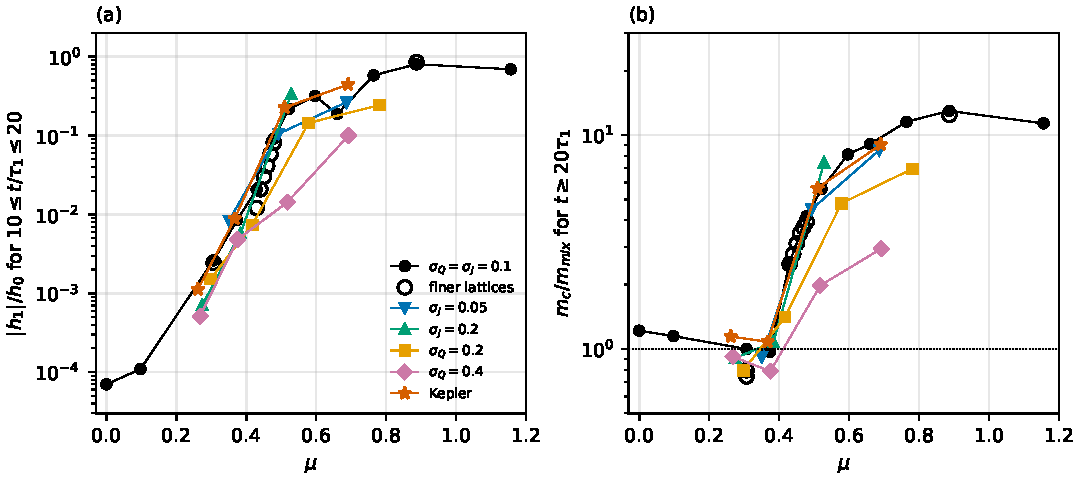
\includegraphics[width=\textwidth]{figuras/bulto_transicion.pdf}}
\caption{All the simulations of the cloud~(\ref{Eq:Pulse}) as functions of the parameter~(\ref{Eq:muDef}). (a) Mean value of $|h_1|/h_0$ over the interval $10\leq t/\tau_1\leq 20$. (b) Mass fraction $m_c$ inside the ellipse~(\ref{Eq:CoreEllipse}) in units of the largest value $m_{mix}$ which is compatible with a gas that is mixed at fixed action (dotted line). The families differ in the widths $\sigma_Q$ and $\sigma_J$ of the cloud (equal to $0.1$ unless otherwise stated) and in the external potential (isochrone unless otherwise stated). The open circles refer to the simulations of the reference family with $N_Q = 100$ or $N_J = 800$. The shaded band indicates the interval $0.43\leq\mu\leq 0.48$.}
\label{Fig:CloudTransition}
\end{figure}

Figure~\ref{Fig:CloudTransition} shows the mean value of $|h_1|/h_0$ over the interval $10\leq t/\tau_1\leq 20$ and the ratio $m_c/m_{mix}$ as functions of $\mu$ for all the simulations. In each family, $|h_1|/h_0$ grows by one to two orders of magnitude within a narrow interval of $\mu$. With the exception of the family with $\sigma_Q = 0.4$, the location of this interval is the same for all the families: all the simulations with $\mu\leq 0.43$ have $|h_1|/h_0\leq 2.1\times 10^{-2}$, and all those with $\mu\geq 0.48$ have $|h_1|/h_0\geq 0.09$. The ratio $m_c/m_{mix}$ behaves in a similar way: it lies between $0.7$ and $1.2$ for all the simulations with $\mu\leq 0.38$, and it is larger than $4$ for all those with $\mu\geq 0.48$ and $\sigma_Q\leq 0.2$. In between, where a core is present whose oscillation is damped, we find $m_c/m_{mix} = 1.4$ for $\sigma_Q = 0.2$ and $\mu = 0.42$, besides the value $2.5$ for the reference family and $\mu = 0.43$; in these two simulations and in the one with $\sigma_J = 0.2$ and $\mu = 0.38$, in which the peak at the circular orbit is narrower than the ellipse, the oscillation of the core is damped with decay times between $4\tau_1$ and $11\tau_1$.

Table~\ref{Tab:Critical} lists, for each family, the largest value of $\mu$ for which the gas relaxes and the smallest one for which the core keeps oscillating. The intervals which are delimited by these values have the common part $0.43\leq\mu\leq 0.48$ for the five families with $\sigma_Q\leq 0.2$, whereas for $\sigma_Q = 0.4$ the transition lies between $\mu = 0.52$ and $\mu = 0.69$. Therefore, for clouds which are compact in angle the critical value $\mu_c$ of the parameter~(\ref{Eq:muDef}) lies between $0.43$ and $0.48$. This interval is determined by the reference family; for the remaining families, in which the masses are more widely spaced, the transition is only bracketed by wider intervals which contain it. A cloud which is wide in angle requires a larger value of $\mu$. The critical value is of order one, as expected from the argument of section~\ref{SubSec:FarRuns}, but this argument does not predict it. Hence, $\mu$ captures the competition between self-gravity and shear for compact clouds, but not the complete dependence on the shape of the cloud. \EJ{A theory of $\mu_c$, including its dependence on $\sigma_Q$, is still missing. Intermediate masses in the families other than the reference one are needed in order to test whether $\mu_c$ is the same for all of them.}

\begin{table}[htp]
\begin{center}
\begin{tabular}{ll|ccc|ccc}
\hline\hline
 & & \multicolumn{3}{c|}{relaxation} & \multicolumn{3}{c}{oscillating core} \\
potential & widths & $\mu$ & $|h_1|/h_0$ & $m_c/m_{mix}$ & $\mu$ & $|h_1|/h_0$ & $m_c/m_{mix}$ \\
\hline
isochrone & $\sigma_Q = \sigma_J = 0.1$ & $0.43$ & $1.2\times 10^{-2}$ & $2.5$ & $0.48$ & $0.091$ & $4.2$ \\
 & $\sigma_J = 0.05$ & $0.35$ & $8.3\times 10^{-3}$ & $0.9$ & $0.49$ & $0.105$ & $4.5$ \\
 & $\sigma_J = 0.2$ & $0.38$ & $5.8\times 10^{-3}$ & $1.1$ & $0.53$ & $0.33$ & $7.4$ \\
 & $\sigma_Q = 0.2$ & $0.42$ & $7.4\times 10^{-3}$ & $1.4$ & $0.58$ & $0.14$ & $4.8$ \\
 & $\sigma_Q = 0.4$ & $0.52$ & $1.4\times 10^{-2}$ & $2.0$ & $0.69$ & $0.10$ & $2.9$ \\
Kepler & $\sigma_Q = \sigma_J = 0.1$ & $0.37$ & $8.8\times 10^{-3}$ & $1.1$ & $0.51$ & $0.23$ & $5.6$ \\
\hline\hline
\end{tabular}
\end{center}
\caption{Bracketing of the transition: for each family, the largest value of $\mu$ for which the gas relaxes and the smallest one for which the core keeps oscillating, together with the mean value of $|h_1|/h_0$ over $10\leq t/\tau_1\leq 20$ and the ratio $m_c/m_{mix}$. In the family with $\sigma_J = 0.05$ ($\sigma_Q = 0.2$, $0.4$) the remaining width is $\sigma_Q = 0.1$ ($\sigma_J = 0.1$). For $\mu = 0.43$ the values refer to $N_Q = 100$; for $N_Q = 25$ they are $2.1\times 10^{-2}$ and $2.5$. Recall that $m_c/m_{mix}$ cannot exceed $F_{max}/\hat{F}_{max}$, which is $4.2$ for $\sigma_Q = 0.4$.}
\label{Tab:Critical}
\end{table}

Regarding the resolution, we note that with $N_Q = 25$ the cloud with $\sigma_Q = 0.1$ is sampled by only four columns of the lattice in the angle variable, two on each side of $Q = 0$ with the relative weights $0.67$ and $0.03$, such that about $600$ of the $10^4$ computational particles carry more than one percent of the largest weight; with $N_Q = 100$ this number is about $2000$. Nevertheless, the results for both lattices agree. For $\mu = 0.31$ we obtain $|h_1|/h_0 = 2.62\times 10^{-3}$ with $N_J\times N_Q = 400\times 25$ and $2.44\times 10^{-3}$ with both $400\times 100$ and $800\times 25$, and the same profile in Fig.~\ref{Fig:CloudState}(a) to within $0.03\,\hat{F}_{max}$. For $\mu = 0.89$ we obtain $|h_1|/h_0 = 0.80$ and $m_c = 0.54$ with $400\times 25$, and $0.85$ and $0.52$ with $400\times 100$. Close to the transition the function $h_1$ depends on the number of particles: for $\mu = 0.43$ its mean value is $2.1\times 10^{-2}$ with $400\times 25$ and $1.2\times 10^{-2}$ with $400\times 100$. This is to be expected, since near the transition the outcome is sensitive to small perturbations, such as those which are due to the discreteness of the particles. However, both simulations lie on the same side of the transition, and the properties of the core agree: $m_c = 0.105$ and $0.103$, and the decay times of its oscillation differ by $20$ percent. \EJ{Not tested yet for the cloud with self-gravity: the dependence on $\Delta r$ (the root mean square radial extension of the core, $0.12$ to $0.17$, is comparable to $\Delta r = 0.1$), on $\Delta t$, and on $N_J$ close to the transition. These tests require new simulations.}

In the Kepler potential the clouds with $M_{gas}/M = 0.01$ and $0.02$ ($\mu = 0.26$ and $0.37$) relax, which is the behavior described by Ref.~\cite{sCjL26} for small data, whereas those with $M_{gas}/M = 0.04$ and $0.08$ ($\mu = 0.51$ and $0.69$) leave an oscillating core. Since $\mu$ grows with the mass, for a cloud of a given shape the relaxation fails above a critical mass, which lies between $M_{gas}/M = 0.02$ and $0.04$ in this case. Note that the core forms at the circular orbit, which is excluded from the support of the initial data considered in Ref.~\cite{sCjL26}. \EJ{A test with a cloud whose support is bounded away from the circular orbit, as in Ref.~\cite{sCjL26}, would show whether a core also forms in that case.}
